% ---------------------------------------------------------------------------
% Author guideline and sample document for EG publication using LaTeX2e input
% D.Fellner, v1.13, Nov 13, 2007

\documentclass{egpubl}

% --- for  Annual CONFERENCE
\VisualComputing % VisualComputing (added by U. Schwanecke, 2021)
%\ThreeDAnimation % 3DAnimation (added by U. Schwanecke, 2020)
%\Seminar % Specialist Seminar (added by U. Schwanecke, 2019)
%\ConferenceSubmission % uncomment for Conference submission
%\ConferencePaper      % uncomment for (final) Conference Paper
%\STAR                 % uncomment for STAR contribution
% \Tutorial             % uncomment for Tutorial contribution
% \ShortPresentation    % uncomment for (final) Short Conference Presentation
%
% --- for  CGF Journal
% \JournalSubmission    % uncomment for submission to Computer Graphics Forum
% \JournalPaper         % uncomment for final version of Journal Paper
%
% --- for  CGF Journal: special issue
% \SpecialIssueSubmission    % uncomment for submission to Computer Graphics Forum, special issue
% \SpecialIssuePaper         % uncomment for final version of Journal Paper, special issue
%
% --- for  EG Workshop Proceedings
% \WsSubmission    % uncomment for submission to EG Workshop
% \WsPaper         % uncomment for final version of EG Workshop contribution
%
%\electronicVersion % can be used both for the printed and electronic version

% !! *please* don't change anything above
% !! unless you REALLY know what you are doing
% ------------------------------------------------------------------------

\PrintedOrElectronic

\usepackage[pdftex]{graphicx} 
\usepackage{t1enc, dfadobe}
%\usepackage[T1]{fontenc}
\usepackage{egweblnk}
\usepackage{cite}

% For backwards compatibility to old LaTeX type font selection.
% Uncomment if your document adheres to LaTeX2e recommendations.
% \let\rm=\rmfamily    \let\sf=\sffamily    \let\tt=\ttfamily
% \let\it=\itshape     \let\sl=\slshape     \let\sc=\scshape
% \let\bf=\bfseries

% end of prologue

\usepackage{blindtext}
\usepackage{caption}
\usepackage{subfigure}
\usepackage{dblfloatfix}
\usepackage{adjustbox}
\usepackage{mathtools}
\usepackage{todonotes}

\usepackage{cleveref}


% ---------------------------------------------------------------------
\captionsetup{labelfont=bf,textfont=it}
\title[Burst Images]%
      {Burst Images}

\author[Sascha Scheid]
    {\parbox{\textwidth}
        {\centering 
			Sascha Scheid
        }
        \\
    {\parbox{\textwidth}
        {\centering RheinMain University of Applied Sciences, Wiesbaden, Germany\\
       }
    }
}
% ------------------------------------------------------------------------

% if the Editors-in-Chief have given you the data, you may uncomment
% the following five lines and insert it here
%
% \volume{36}   % the volume in which the issue will be published;
% \issue{1}     % the issue number of the publication
% \pStartPage{1}      % set starting page


%-------------------------------------------------------------------------
\begin{document}

%-------------------------------------------------------------------------
% uncomment for using teaser (comment if you don't want a teaser)
\teaser{
    \hspace{\fill}
    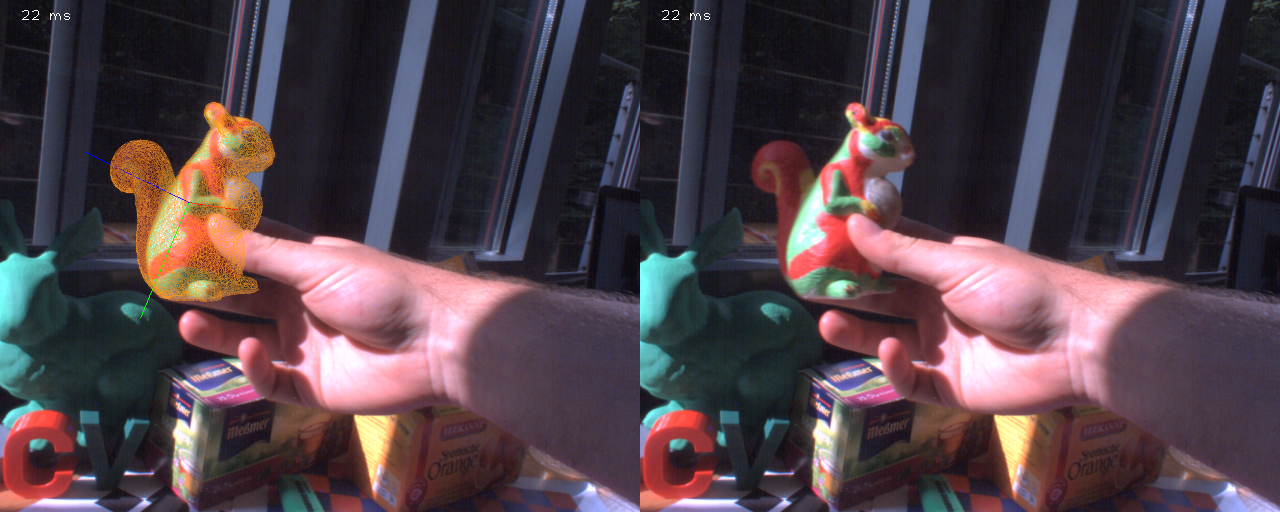
\includegraphics[width=0.9\linewidth]{images/ModelbasedTrackingExample.png}
    \hspace{\fill}
    \centering
    \caption{Best teaser image you can provide \ldots}
    \label{fig:teaser}
}


%-------------------------------------------------------------------------
\maketitle


%-------------------------------------------------------------------------
\begin{abstract}
Some informative abstract \ldots
\blindtext
\end{abstract}  


%-------------------------------------------------------------------------
\section{Introduction}
\label{sec:introduction}

Burst photography is a technique in which a series of photographs is taken quickly in succession.
This can be useful in a variety of situations, such as capturing action or movement, 
or to create a sense of motion. In digital photography, burst images are stored as a 
sequence of image files, typically in a format such as JPEG or RAW.

High Dynamic Range (HDR) is a technique used to improve the dynamic range of an image, 
which is the range of luminance or brightness levels that can be captured in a photograph. 
The dynamic range of a scene can often be greater than what a camera is able to capture 
in a single image, resulting in lost detail in the highlights or shadows. 
HDR techniques can be used to extend the range of luminance in an image, 
resulting in more detail and a more realistic representation of the scene.

One way that burst photography and HDR techniques can be used together
is to capture a series of photographs with different exposures in a burst, and then combine 
the exposures into a single HDR image using software. This can be particularly useful in 
low-light situations, where the camera may struggle to capture a wide range of luminance 
levels in a single exposure. By capturing multiple exposures and combining them into an 
HDR image, it is possible to extend the dynamic range and capture more detail in both the 
highlights and shadows.

Mobile cameras can have several constraints in low light situations, including:

\begin{itemize}
    \item Low sensitivity: Mobile cameras often have smaller sensors compared 
          to DSLR or mirrorless cameras, which can result in lower sensitivity 
          to light. This can make it difficult to capture usable images in low l
          ight conditions without using long exposures or high ISO values, 
          which can introduce noise and other artifacts.
    
    \item Limited dynamic range: Mobile cameras can have limited dynamic range, 
          which can make it difficult to capture both the shadow and highlight 
          details in a scene. This can result in underexposed or overexposed 
          areas in the image, and can be particularly challenging in low light 
          conditions where the range of luminance values is often greater.
    
    \item Motion blur: Long exposures are often necessary in low light conditions, 
          which can result in motion blur if the camera or the subject is moving. 
          This can be particularly problematic for handheld shots or when photographing 
          moving subjects.
\end{itemize}

To address these constraints, several techniques can be used to improve the performance 
of mobile cameras in low light conditions. These include:

\begin{itemize}
    \item Noise reduction: Noise reduction algorithms can be used to reduce the noise 
          introduced by high ISO values or long exposures. These algorithms can smooth 
          out the image while preserving edges and other important details.

    \item High dynamic range techniques: HDR techniques, such as burst photography 
          and computational photography, can be used to extend the dynamic range of mobile 
          cameras and capture more detail in both the shadow and highlight areas of an image.
    
    \item Image stabilization: Image stabilization technologies, such as optical image 
          stabilization or electronic image stabilization, can be used to reduce the 
          effects of camera shake or subject movement during long exposures.
\end{itemize}
    
While there are still limitations to the capabilities of mobile cameras compared to larger, 
more specialized cameras, advances in technology and image processing algorithms are 
continually improving the quality and performance of mobile cameras in a variety of 
lighting conditions.


%-------------------------------------------------------------------------
\section{Related Work}
\label{sec:related_work}

The HDR+ algorithm is a computational photography technique developed by Google for use 
in the Google Pixel smartphone. It is designed to capture high dynamic range images using 
burst photography. The algorithm uses computational techniques to extend the dynamic range 
of the captured images, rather than relying on multiple exposures as in traditional 
HDR techniques, in which a rapid sequence of images at different exposures is captured.
The captured images are merged to create a single HDR image. The HDR+ algorithm was developed 
to improve the quality and dynamic range of images captured on mobile devices, particularly in 
low-light conditions. The HDR+ algorithm consists of several steps, which are outlined in detail 
in \cite{Hasinoff2016burst}. In brief, the steps are as follows:

\begin{enumerate}
    \item Burst capture: A sequence of raw images is captured. In contrast to the classic 
          multi-exposure approach, each image will be underexposed and all images have the
          same exposure. An image bursts consists of two to eight single images.
    \item Image alignment: The sharpest image of the first three images in the burst is 
          selected as reference image and the remaining images in the burst are aligned 
          to it. This corrects for any movement or misalignment between frames.
    \item Image merging: The aligned raw images are merged to create a single intermediate 
          raw image that will then be further processed.
    \item Finishing: The merged image undergoes a set of operations including general
          correction, demosaicking and tone mapping. The most important operation is
          dynamic range compression which reduces the contrast between light and dark
          areas while preserving local contrast. To do so, the local tone mapping method
          \textit{exposure fusion} was used, which blends together the best parts of
          differently exposed images. As there is only one merged image left, the ones 
          to blend are created synthetically from the merged image.

\end{enumerate}


%-------------------------------------------------------------------------
\section{Approach}
\label{sec:approach}

\begin{itemize}
      \item Provide more details
      \begin{itemize}
            \item why does the git project not work?
            \item overall architecture
            \item how does the script work?
            \item folder structure
            \item configuration
      \end{itemize}
\end{itemize}

\cite{Brooks2016git} has implemented the image processing pipeline described in \cref{sec:related_work}. To do this, 
he uses Halide, a programming language embedded in C++ that allows efficient image processing 
pipelines to be implemented with little effort. Halide itself requires LLVM to compile. 
Unfortunately, the project has not been actively maintained for quite some time and 
since new versions of Halide and LLVM have been released in the meantime, some of which were 
not backwards compatible, the project could not be compiled out of the box. After many hours of 
trial and error, the project was able to compile with version 10 of both Halide and LLVM. 
To get a reproducible executable version of \cite{Brooks2016git}, a Docker image was created that 
contains the application and runs it on container startup. To improve efficiency, a script was created 
that starts processing all image bursts that are stored inside a bursts directory, which is shared
with the Docker container, in parallel. \Cref{fig:architecture} shows the architecture described above.

\begin{figure}
    \hspace{\fill}
    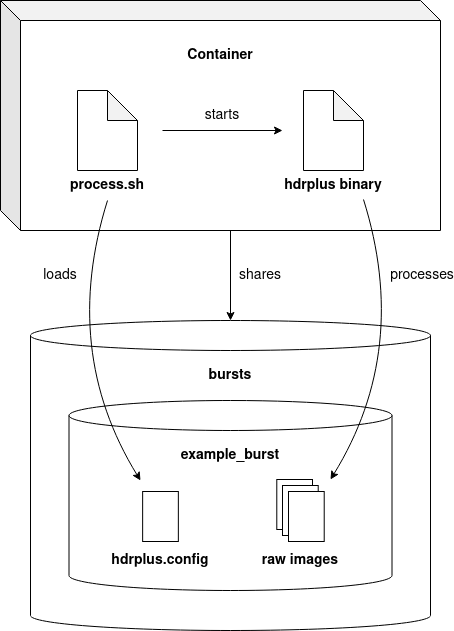
\includegraphics[width=0.9\linewidth]{images/architecture.png}
    \hspace{\fill}
    \centering
    \caption{Architecture of the dockerized application}
    \label{fig:architecture}
\end{figure}

%-------------------------------------------------------------------------
\section{Experiments}
\label{sec:Experiments}

\begin{itemize}
      \item Insert images
      \item Compare raw vs processed
      \item Show examples for scenarios:
      \begin{itemize}
            \item Low light noise reduction
            \item Improving contrast / dynamic range
            \item Improving overall colors
      \end{itemize}
      \item Show fails
\end{itemize} 

%-------------------------------------------------------------------------
\section{Conclusions}

\begin{itemize}
      \item Are there scenes that are very easy or hard to improve?
      \item Advantages:
      \begin{itemize}
            \item (Revived dead open source project, yay)
            \item Portable solution because Docker
            \item Parallel processing of multiple bursts
            \item Not as much work as manually editing bracketed bursts in photoshop
      \end{itemize}
      \item Drawbacks:
      \begin{itemize}
            \item Long initial compiling time when building Docker image
            \item Overhead because Docker
            \item Ease of use: command-line only, adjusting config by editing a file
      \end{itemize}
      \item Future:
      \begin{itemize}
            \item Use case: Photographer wanting HDR images, but does not want to spend
                  hours in photoshop
            \item Providing GUI:
            \begin{itemize}
                  \item Hide docker and script execution for non-nerdy users
                  \item Select burst folders to processes
                  \item Adjust gain and compress parameters by slider per folder
                  \item Start processing of selected folders via button click
                  \item Show result images when finished
            \end{itemize}
      \end{itemize}
\end{itemize}
\label{sec:conclusion}


%-------------------------------------------------------------------------
\section{Acknowledgements}
\label{sec:acknowledgements}
\begin{itemize}
      \item Cat
      \item Elementary school teacher
      \item Ex girlfriend
      \item Random dude at the bar who bought a round
\end{itemize}


%-------------------------------------------------------------------------
%\bibliographystyle{eg-alpha}
\bibliographystyle{eg-alpha-doi}
\bibliography{paper-bib}

\end{document}